% TLDR: ICML 2027 submission draft (anonymous): do LLM judges of formal specification coverage beat a constant forecast of the human rating distribution?
% Draft started 11-24-2026. Gaps for pending results are marked \TODO{...} (red) with a date.
\documentclass{article}
\usepackage{microtype}
\usepackage{graphicx}
\usepackage{subcaption}
\usepackage{booktabs}
\usepackage{xcolor}
\usepackage{hyperref}
\newcommand{\theHalgorithm}{\arabic{algorithm}}
\usepackage{icml2027}
\usepackage{amsmath}
\usepackage{amssymb}
\usepackage{mathtools}
\usepackage{amsthm}
\usepackage{float}
\usepackage[capitalize,noabbrev]{cleveref}

\theoremstyle{plain}
\newtheorem{proposition}{Proposition}
\theoremstyle{remark}
\newtheorem{remark}{Remark}

% Dated placeholder for a result that is not in yet (visible in red; remove before submission).
\newcommand{\TODO}[1]{{\color{red}\textbf{[TODO #1]}}}
\newcommand{\RPS}{\mathrm{RPS}}
\newcommand{\CE}{\mathrm{CE}}
\newcommand{\TVD}{\mathrm{TVD}}

\icmltitlerunning{Does the Judge Beat the Constant?}

\begin{document}

\twocolumn[
  \icmltitle{Does the Judge Beat the Constant?\\
  Evaluating LLM Judges of Formal Specification Coverage with Proper Scores}

  \begin{icmlauthorlist}
    \icmlauthor{Anonymous Authors}{anon}
  \end{icmlauthorlist}
  \icmlaffiliation{anon}{Anonymous Institution}
  \icmlcorrespondingauthor{Anonymous Authors}{anonymous@example.com}
  \icmlkeywords{LLM judges, proper scoring rules, evaluation, formal verification, Lean}
  \vskip 0.3in
]

\printAffiliationsAndNotice{}

% !TEX root = 00_main.tex
% TLDR: Abstract with the headline numbers of experiments 22, 25 and the earlier-panel result; pending result marked.
\begin{abstract}
Large language model (LLM) judges are usually validated by their correlation with human ratings.
We ask a stricter question for judges of formal specification coverage (FSC) of Lean 4 formalizations: does the judge's forecast of the human rating distribution of an artifact beat a constant forecast, the average human rating distribution of the training tasks, on held-out tasks?
We score forecasts with the ranked probability score (RPS) and cross-entropy (CE), both strictly proper, and the total variation distance (TVD), and report Spearman and Pearson correlation only as secondary columns.
On 75 artifacts from 25 tasks (195 expert ratings), a judge with test Spearman $0.83$ has test RPS $0.195$ against $0.184$ for the constant (paired difference $+0.012$, 95\% interval $[-0.090,+0.109]$), and a leniency bias of $+0.18$ on the normalized $[0,1]$ rating scale accounts for 55\% of its test squared error and is invisible to correlation.
Pooling with 100 new artifacts from 25 further tasks (247 ratings) narrows the absolute width of the RPS interval to $0.60\times$ to $0.64\times$ of the old-only width, yet against the set-aware constant neither frontier judge is clearly better (RPS differences $+0.002$ and $-0.018$) and both overscore the old artifacts by about half a point.
An earlier panel of 24 judge series scored on the corrected-label set has none significantly better than the constant after calibration.
A judge built for this question on the pooled ratings (CE-fitted calibration of two frontier judges' scores and a new prompt) has, on 20 held-out tasks (70 artifacts), RPS $0.075$ against $0.110$ for the set-aware constant, CE $0.97$ against $1.19$ and TVD $0.35$ against $0.48$; the paired RPS difference is $-0.035$ with 95\% interval $[-0.076,+0.002]$, so under our pre-registered rule the verdict is promising, not works.
\end{abstract}

% !TEX root = 00_main.tex
% TLDR: Motivation, the constant-forecast question, what we do, contributions (one per experiment).
\section{Introduction}
\label{sec:intro}
A Lean formalization of a program can prove every theorem it states and still omit a property the program must satisfy.
Whether a formalization states what is required is its \emph{formal specification coverage} (FSC); a proof assistant does not check it, so people rate it, and rating at scale is expensive.
LLM judges are the usual substitute~\citep{zheng2023judging,gu2024survey}, and a judge is usually validated by its correlation with human ratings~\citep{liu2023geval,kim2024prometheus}.

Correlation is a weak certificate.
Spearman and Pearson correlation are blind to a constant shift of the judge's scores and, for Pearson, to their scale, and Spearman additionally ignores everything but their order (\cref{sec:setup}).
A judge that is a full rating point too lenient on every artifact has correlation $1$ with a judge that is exactly right.
Our question is therefore one that correlation cannot answer: \emph{given a new task, does the judge predict the distribution of ratings human experts give to its artifacts better than a constant forecast that ignores the artifact?}
The constant is the average human rating distribution of the training tasks.
It is the cheapest honest baseline, and any claim that a judge ``works'' on held-out tasks should beat it.

We score each judge's forecast of the human rating distribution with the ranked probability score (RPS), cross-entropy (CE) and total variation distance (TVD; \cref{sec:setup}); RPS and CE are strictly proper, so they are minimized in expectation only by the true distribution, and we put all three first in every table.
Spearman and Pearson correlation are secondary columns.
All intervals resample whole tasks, since artifacts of one task are not independent.
Data are 75 old artifacts from 25 tasks (195 expert ratings) and 100 new artifacts from 25 other tasks (247 ratings returned so far), plus an earlier judge panel scored against corrected labels (\cref{sec:data}).

\paragraph{Contributions.}
Each is a result from a pre-registered or dated experiment and stays negative where the data are negative.
\begin{enumerate}
\item \textbf{High correlation, no gain over the constant (\cref{sec:exp22}).} The judge selected for its correlations (Spearman $0.64$, $0.88$, $0.83$ on train, validation, test tasks) has test RPS $0.195$ against $0.184$ for the constant; $55\%$ of its test squared error is a leniency bias that correlation discards.
\item \textbf{Training objective (\cref{sec:exp22}).} Across 1{,}000 random task splits, mixtures of judges fitted by cross-entropy beat mixtures fitted by Pearson correlation on cross-entropy and total variation distance, tie on RPS, and lose on correlation.
\item \textbf{More human ratings (\cref{sec:exp25}).} Doubling the tasks to 50 narrows the absolute width of the RPS interval to $0.60\times$ to $0.64\times$ of the old-only width, but it measures the judge better; it does not make the judge better: against the set-aware constant neither frontier judge is clearly better (both intervals contain $0$), and pooling two sets with different rating levels manufactures an apparent gain.
\item \textbf{An earlier panel (\cref{sec:cert}).} On the corrected-label set none of three headline judge series beats the constant (raw RPS $0.217$ to $0.271$ against $0.174$), their Spearman point estimates are negative ($-0.21$ to $-0.35$; the interval excludes $0$ only for Qwen3-Coder), and after calibration none of 24 series is significantly better than the constant.
\item \textbf{A judge that works (\cref{sec:exp27}).} We pre-registered, before any run, what ``works'' means and how a judge is built on old and new ratings with fixed task splits. \TODO{11-24-2026: held-out test result of this experiment.}
\end{enumerate}

% !TEX root = 00_main.tex
% TLDR: LLM judges, proper scores for ordinal forecasts, evaluation validity, autoformalization, selection bias.
\section{Related Work}
\label{sec:related}
\paragraph{LLM judges.}
\citet{zheng2023judging} measure agreement between LLM judges and human preferences and document position, verbosity and self-enhancement biases; \citet{wang2023fair} study position bias in particular; \citet{gu2024survey} survey the area.
G-Eval and Prometheus score outputs with a rubric and report their correlation with human ratings~\citep{liu2023geval,kim2024prometheus}.
We study a different target (formal statements checked against a reference), and a different standard: held-out performance against a constant forecast, not agreement alone.

\paragraph{Proper scores for ordinal forecasts.}
Strictly proper scoring rules reward a forecaster only for reporting its true belief~\citep{gneiting2007strictly,gneiting2014probabilistic}.
The ranked probability score (RPS) extends the Brier score~\citep{brier1950verification} to ordered categories~\citep{epstein1969scoring,murphy1971note}.
We use it as the primary metric and cross-entropy and total variation distance as co-primary ones; the novelty is not the scores but the combination with a constant forecast, task-cluster bootstrap intervals and the human rating distribution as the target.

\paragraph{Fitting judges: correlation versus likelihood.}
A concurrent study (cited anonymously for review) argues, on other judge panels, that judges should be fitted by cross-entropy rather than correlation and reports lower held-out RPS for cross-entropy-fitted calibration in all 35 judge-by-budget cells~\citep{anon2026corrce}.
That work is about the fitting objective on general judge panels; this paper is about the verdict on a specific judge family (FSC) against a constant forecast, with a new human-rating collection, and it reports where the earlier direction holds only weakly (\cref{sec:cert}).

\paragraph{Autoformalization and specification coverage.}
Autoformalization benchmarks translate informal mathematics into formal statements and face the same question, whether a statement faithfully covers what was meant~\citep{wu2022autoformalization,azerbayev2023proofnet,zheng2022minif2f}; Lean~4~\citep{moura2021lean4} checks proofs but not coverage.
We take the VeriBench benchmark~\citep{veribench2026} as the source of tasks and use its human-rating study to evaluate judges.

\paragraph{Selection bias and dependent data.}
Repeated model selection biases subsequent performance estimates~\citep{cawley2010overfitting}; we select on validation tasks and score once on held-out tasks (\cref{sec:exp27}).
Artifacts of one task share inputs, so we resample tasks, in the spirit of the cluster bootstrap~\citep{field2007bootstrapping}.

% !TEX root = 00_main.tex
% TLDR: Target, forecasts, metrics (RPS, CE, TVD primary; Spearman, Pearson secondary), the constant forecast and its set-aware version, intervals.
\section{Problem Setup and Metrics}
\label{sec:setup}
\paragraph{Target.}
For a task $t$, let an \emph{artifact} be a candidate Lean formalization $a$ of the task's Python program.
A rater sees the Python source, the reference Lean file and the artifact, and gives an integer rating $r\in\{0,\dots,5\}$ for how fully the artifact's theorem statements cover the reference's (rubric in \cref{app:rubric}; proofs are not rated).
The \emph{human rating distribution} $p^*_i$ of artifact $i$ is the distribution of ratings a qualified expert would give; we observe $m_i\ge 2$ of its samples.
A \emph{judge} outputs a forecast $q_i$, a probability vector over the six ratings.
Each judge call returns an integer; the forecast is the histogram of the judge's repeated calls on the artifact, floored once at $\epsilon=10^{-6}$ and renormalized (in \cref{sec:cert} the histogram over $0,\dots,5$ is smoothed with a Laplace count of $0.5$ instead).

\paragraph{Primary metrics (lower is better).}
With $Q_c=\sum_{r\le c}q_r$, the normalized ranked probability score of a forecast against one rating $r$ is
\begin{equation}
  S(q,r)=\tfrac15\sum_{c=0}^{4}\bigl(Q_c-\mathbf 1\{r\le c\}\bigr)^2\in[0,1].
\end{equation}
\emph{RPS} is the mean of $S(q_i,r)$ over the ratings of artifact $i$, then over artifacts with equal weight.
\emph{CE} is the mean cross-entropy $-\log q_i(r)$ of the observed ratings, and \emph{TVD} is $\tfrac12\sum_r|q_i(r)-\hat p_i(r)|$ against the empirical rating histogram $\hat p_i$.
RPS and CE are proper; TVD is a distance to a noisy empirical histogram and is a diagnostic.
\Cref{app:derivations} shows $\mathbb E\,S(q,R)=D(q,p^*)+U(p^*)$, with $D=\tfrac15\sum_c (Q_c-P_c)^2$ the distribution error and $U$ the irreducible disagreement of the raters.
Both CE and RPS are minimized only at $q=p^*$.
CE depends strongly on the floor $\epsilon$ for judges that output few distinct scores (\cref{app:floor}); RPS barely moves, which is why RPS is the headline.

\paragraph{Secondary metrics.}
\emph{Spearman} and \emph{Pearson} correlation between the judge's mean score and the human mean score per artifact.
Both are invariant to $\mu\mapsto a+b\mu$ with $b>0$ (Pearson) or to any increasing map (Spearman).
For Pearson the mean squared error splits exactly as $\mathrm{MSE}=\text{bias}^2+(s_x-s_y)^2+2s_xs_y(1-r)$: correlation sees only the last term (\cref{app:derivations}).

\paragraph{The constant forecast.}
The \emph{constant} forecast gives every held-out artifact the pooled human rating distribution of the training tasks (leave-one-task-out when no split is fixed).
When two artifact sets with different rating levels are pooled, the \emph{set-aware constant} uses each set's own training distribution, computed leave-one-task-out inside the set; it is the fair baseline for pooled results (\cref{sec:exp25}).

\paragraph{Uncertainty.}
Unless stated, intervals are $95\%$ percentile intervals of a task-cluster bootstrap (whole tasks resampled with replacement; $10{,}000$ draws, except the earlier-panel experiment of \cref{sec:cert} and the ``Test, ordinary'' row of \cref{tab:exp22}, which use $2{,}000$).
A difference between a judge and a baseline is paired on the same resampled tasks.
\emph{Decision rule:} a judge \emph{beats} a baseline only if the paired RPS interval lies entirely below $0$.

% !TEX root = 00_main.tex
% TLDR: Human-rating setup and the three data sets; table of sizes.
\section{Human Ratings, Data and Judges}
\label{sec:data}
\paragraph{Rating protocol.}
Raters score the coverage of the reference's theorem statements by the artifact's statements on a 0 to 5 rubric, with an adjustment for theorem spam; between two adjacent scores they pick the lower unless they can justify the higher (\cref{app:rubric}).
Each rater has a personal rating sheet with identifiers prefilled; raters state whether AI assistance was used, and the sheets record minutes spent and confidence.
Per-artifact human distributions are noisy: most artifacts have two to three ratings.

\paragraph{Data sets.}
\Cref{tab:data} lists the three sets.
The \emph{old set} (75 artifacts) was rated earlier by a three-expert subset and its judges were developed on it; it has a fixed split of $10/5/10$ train, validation and test tasks.
The \emph{new set} (100 artifacts) has four frontier coding agents on each of 25 tasks, each in its vendor's own harness, with no task shared with the old set; its ratings arrive in waves, and the numbers here use the 247 ratings returned by 11-24-2026 (read at 10:38 PST for \cref{sec:exp25} and again at 12:58 PST for \cref{sec:exp27}, 247 ratings each time), from 5 raters, with 73\% of them equal to 5.
The \emph{corrected-label set} belongs to an earlier judge panel and has 59 artifacts from 20 tasks, 4.5 ratings each, under a corrected rubric.

\begin{table}[t]
\caption{Data sets. Ratings of the new set are a first wave (247 of 3{,}300 sheet rows returned).}
\label{tab:data}
\centering\small
\resizebox{\linewidth}{!}{\begin{tabular}{lrrrl}
\toprule
Set & Tasks & Artifacts & Ratings & Used in\\
\midrule
Old & 25 & 75 & 195 & \cref{sec:exp22,sec:exp25}\\
New & 25 & 100 & 247 & \cref{sec:exp25,sec:exp27}\\
Pooled & 50 & 175 & 442 & \cref{sec:exp25,sec:exp27}\\
Corrected labels & 20 & 59 & 4.5 per artifact & \cref{sec:cert}\\
\bottomrule
\end{tabular}}
\end{table}

\paragraph{Judges.}
The \emph{H2 judge} prompt gives the rater instructions and four rated demonstrations from other tasks, and asks for one integer score per call.
We evaluate GPT-6 Sol, GPT-6 Astra, Gemini 4 Argon and Claude Opus 5.5, each with three calls per artifact (the selected judge pairs two models for six calls).
Harness and model differ between old and new artifacts for two judges (\cref{app:harness}); we say where pooled rows mix harnesses.
The earlier panel has gpt-5.3-codex, claude-opus-4-7 and Qwen3-Coder-30B-A3B-Instruct under four prompts each, gpt-4o-mini under two, and an edit-distance and a random control, counted per family (24 series).

% !TEX root = 00_main.tex
% TLDR: Four results (exp 22, exp 25, earlier panel exp 67) and the pending judge-building experiment (exp 27).
\section{Experiments}
\label{sec:experiments}
Every number below is copied from the results file of its experiment, or recomputed from the anonymized data by a script named there (\cref{app:trace}); tables list RPS, CE and TVD first and correlations last.

\subsection{Does the selected judge beat the constant?}
\label{sec:exp22}
We re-score, on the full panel, the judge that had been selected for its correlations: GPT-6 Sol and Claude Opus 5.5 (H2 prompt, three calls each) on the old set, with the canonical $10/5/10$ task split.
The constant is the training-task rating distribution.
\Cref{tab:exp22} shows that correlation jumps between splits (Spearman $0.64$, $0.88$, $0.83$) while test RPS ($0.195$) is no better than the constant ($0.184$): the paired difference is $+0.012$ with interval $[-0.090,+0.109]$.
On the 24 ordinary test artifacts (two test tasks have placeholder references) the judge is nominally worse, RPS $0.223$ against $0.178$, and test Spearman falls from $0.83$ to $0.65$ with interval $[-0.17,+0.92]$.
Cross-entropy of the judge is far above the constant on every split, but it is floor-dependent (\cref{app:floor}); the judge's test TVD ($0.628$) is below the constant's ($0.665$), but the paired difference ($-0.037$, $[-0.209,+0.126]$) includes $0$.

\begin{table*}[t]
\caption{The selected judge (GPT-6 Sol and Claude Opus 5.5, H2 prompt, 6 calls) by split on the old set. RPS has the task-cluster bootstrap 95\% interval; the constant is the training-task distribution. RPS, CE and TVD first, correlations last.}
\label{tab:exp22}
\centering\small
\begin{tabular}{lrccccrr}
\toprule
Split (artifacts / tasks / ratings) & RPS [95\%] & Const. RPS & CE & Const. CE & TVD & Spearman & Pearson\\
\midrule
Train (30 / 10 / 78) & 0.179 [0.118, 0.255] & 0.174 & 7.99 & 1.74 & 0.583 & 0.64 & 0.66\\
Validation (15 / 5 / 39) & 0.129 [0.056, 0.207] & 0.167 & 5.47 & 1.78 & 0.500 & 0.88 & 0.86\\
\textbf{Test} (30 / 10 / 78) & \textbf{0.195} [0.125, 0.267] & \textbf{0.184} & 8.31 & 1.81 & 0.628 & 0.83 & 0.86\\
Test, ordinary (24 / 8 / 66) & 0.223 [0.141, 0.297] & 0.178 & 8.95 & 1.84 & 0.681 & 0.65 & 0.83\\
All (75 / 25 / 195) & 0.176 [0.133, 0.221] & 0.176 & 7.62 & 1.77 & 0.584 & 0.76 & 0.77\\
\bottomrule
\end{tabular}
\end{table*}

\paragraph{Why correlation missed it.}
\Cref{tab:mse} splits the test mean squared error of the judge's mean score.
Bias and scale mismatch, which correlation discards, are $55\%$ and $2\%$ of the test error and $58\%$ and $16\%$ of the ordinary-test error.
The judge overscores the test artifacts by $+0.18$ on the $[0,1]$ scale ($0.653$ against $0.472$).
On the 8-judge frontier pool the single judge with the lowest test RPS (GPT-6 Sol with the H0 prompt, $0.191$) has lower correlations ($0.66$ Pearson, $0.59$ Spearman) than the H2 judges, which have higher RPS ($0.84$ to $0.87$ Pearson), and none of the single judges beats the constant ($0.184$); all three frontier judges added later share the $+0.17$ bias of the H2 prompt.

\begin{table}[t]
\caption{Split of the mean squared error (MSE) of the selected judge's mean score on the $[0,1]$ scale. Correlation sees only the last column.}
\label{tab:mse}
\centering\small
\begin{tabular}{lcccc}
\toprule
Split & MSE & Bias$^2$ & Scale & $2s_xs_y(1{-}r)$\\
\midrule
Train & 0.066 & 8\% & 0.5\% & 91\%\\
Validation & 0.034 & 28\% & 2\% & 70\%\\
Test & 0.060 & \textbf{55\%} & 2\% & 43\%\\
Test, ordinary & 0.072 & \textbf{58\%} & 16\% & 26\%\\
\bottomrule
\end{tabular}
\end{table}

\paragraph{Training objective.}
Does fitting judges by cross-entropy instead of correlation help?
Over $1{,}000$ random $20/5$ task splits of the old set, with mixtures of the eight judges weighted on the training tasks, the mixture trained by cross-entropy (\emph{CE-trained}) and the mixture trained by Pearson correlation (\emph{Pearson-trained}) are tied on RPS (Pearson-trained minus CE-trained: $+0.005$, $[-0.003,+0.014]$), CE-trained is clearly better on CE ($+0.74$, $[+0.30,+1.28]$) and TVD ($+0.028$, $[+0.005,+0.051]$), and Pearson-trained has the higher correlations (Spearman $+0.079$, Pearson $+0.049$).
On the single canonical split an RPS-trained mixture beats the Pearson-trained one on test RPS ($0.144$ against $0.169$, $p=0.007$), but that interval conditions on the fitted weights and the 1{,}000-split tie is the more reliable reading.
The two objectives are not separated by RPS; they are separated by what each is blind to.

\subsection{Do more human ratings help?}
\label{sec:exp25}
We pool the old (75 artifacts, 195 ratings) and new (100 artifacts, 247 ratings) sets: 50 tasks, 442 ratings, scored by GPT-6 Astra and Claude Opus 5.5 under the frozen H2 prompt with the old four demonstrations.
\Cref{tab:exp25} gives the metrics.
The absolute width of the RPS interval of the pooled set is $0.60\times$ (Astra) and $0.64\times$ (Opus) of the old-only width (relative to the estimate itself it does not shrink, because the new set has a lower RPS level), the Spearman interval is $0.41\times$ and $0.39\times$ (partly because the sets are mixed; ranks taken inside each set give $0.66\times$ and $0.72\times$), and the spread of the estimate falls from $k=10$ to $k=25$ tasks (\cref{fig:lc}).
All three pre-registered checks of a better \emph{evaluation} are met.

\begin{table*}[t]
\caption{Old, new and pooled sets (task-cluster bootstrap 95\% intervals, $10{,}000$ draws). Constant = pooled human distribution (leave-one-task-out); on the pooled row it is computed over both sets together. RPS, CE and TVD first.}
\label{tab:exp25}
\centering\small
\begin{tabular}{llcccccrr}
\toprule
Judge & Set & RPS [95\%] & Const. RPS & CE [95\%] & TVD [95\%] & Spearman [95\%] & Pearson [95\%]\\
\midrule
GPT-6 Astra & old & 0.207 [0.150, 0.269] & 0.183 & 8.50 [6.92, 9.95] & 0.629 [0.522, 0.727] & 0.65 [0.35, 0.88] & 0.65 [0.29, 0.87]\\
 & new & 0.055 [0.032, 0.080] & 0.070 & 3.42 [2.08, 4.84] & 0.253 [0.157, 0.355] & 0.59 [0.32, 0.78] & 0.81 [0.65, 0.90]\\
 & pooled & 0.120 [0.087, 0.158] & 0.164 & 5.60 [4.40, 6.80] & 0.414 [0.329, 0.500] & 0.79 [0.66, 0.88] & 0.78 [0.60, 0.89]\\
Claude Opus 5.5 & old & 0.179 [0.135, 0.223] & 0.183 & 8.10 [6.63, 9.49] & 0.600 [0.498, 0.696] & 0.77 [0.55, 0.90] & 0.78 [0.61, 0.89]\\
 & new & 0.041 [0.027, 0.056] & 0.070 & 2.42 [1.56, 3.29] & 0.193 [0.128, 0.258] & 0.65 [0.41, 0.80] & 0.90 [0.74, 0.95]\\
 & pooled & 0.101 [0.074, 0.131] & 0.164 & 4.85 [3.81, 5.98] & 0.368 [0.292, 0.448] & 0.86 [0.77, 0.91] & 0.86 [0.77, 0.92]\\
\bottomrule
\end{tabular}
\end{table*}

\begin{figure*}[t]
\centering
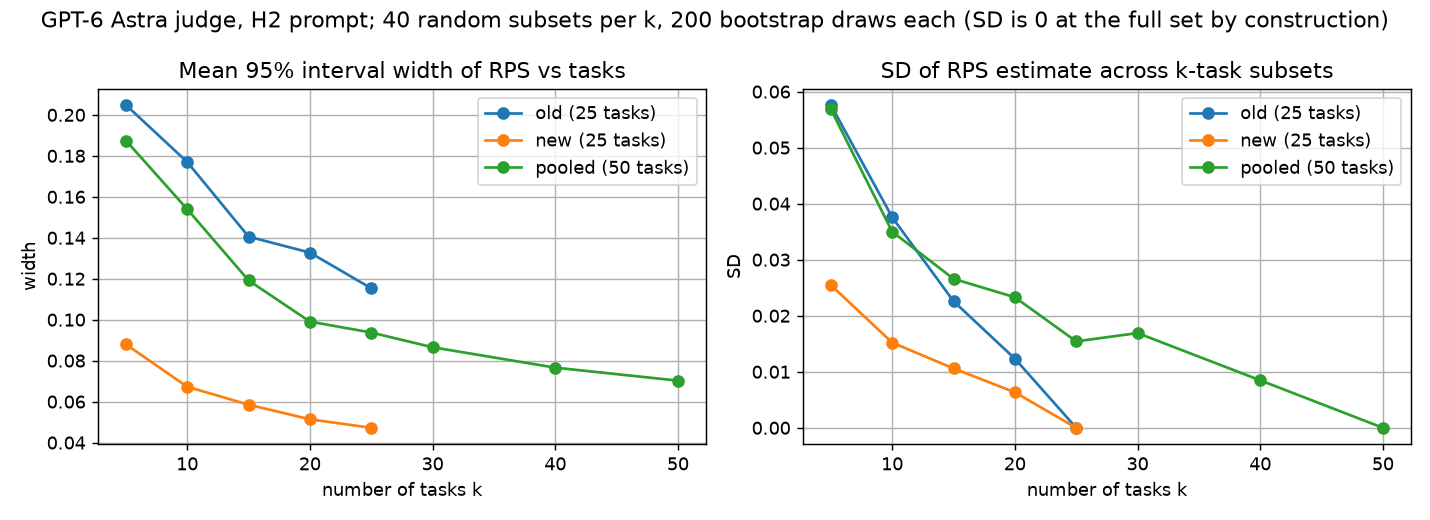
\includegraphics[width=0.85\textwidth]{figures/learning_curve_exp25.png}
\caption{Interval width and spread of the RPS estimate against the number of tasks $k$ (GPT-6 Astra, H2 prompt; 40 random task subsets per $k$, 200 bootstrap draws each). The spread is zero at the full set by construction. The width keeps falling past 25 tasks but slowly after about 30.}
\label{fig:lc}
\end{figure*}

\begin{figure*}[t]
\centering
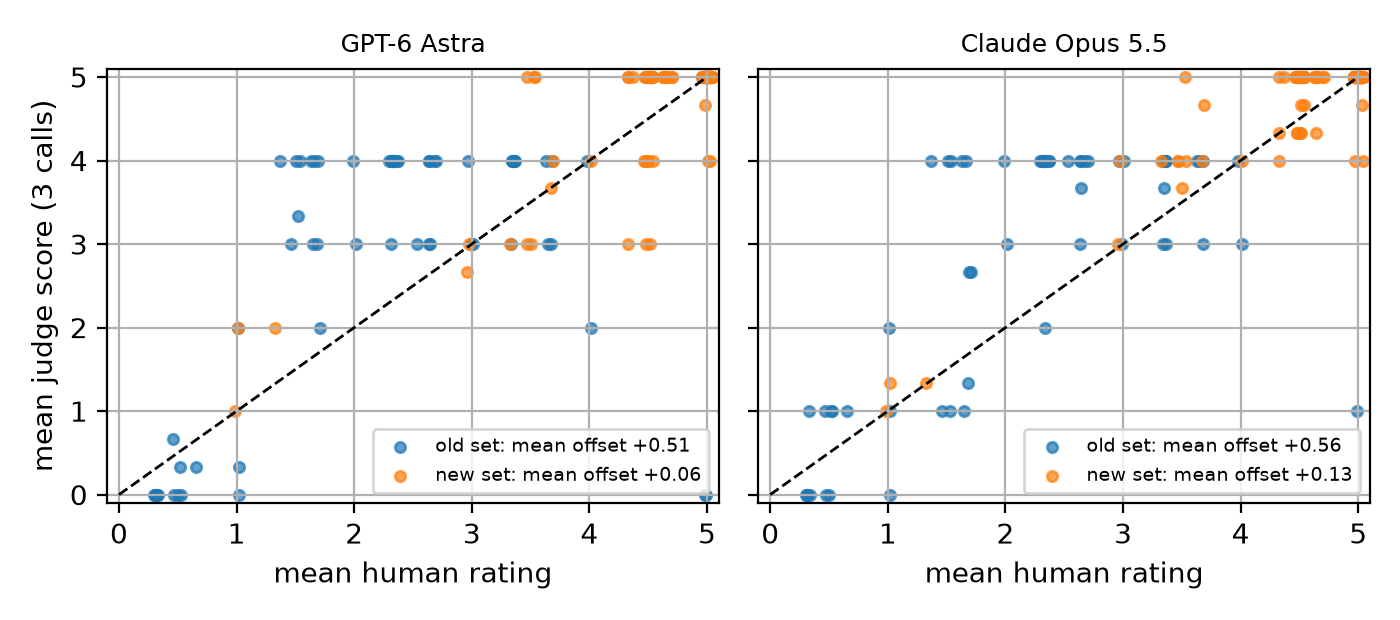
\includegraphics[width=0.8\textwidth]{figures/scatter_judge_vs_human.png}
\caption{Mean judge score (three calls, H2 prompt) against mean human rating for each of the 75 old and 100 new artifacts; dashed line is equality. The mean offset (judge minus human) is $+0.51$ and $+0.56$ on the old set but $+0.06$ and $+0.13$ on the new set, where human ratings are mostly 5s. Points are jittered by up to $0.04$ in $x$.}
\label{fig:scatter}
\end{figure*}

\paragraph{But the judge is not better.}
The pooled rows look like a large gain over the constant ($0.120$ and $0.101$ against $0.164$), but that constant mixes an old set with mean rating $2.63$ of $5$ and a new set that is mostly 5s (mean $4.57$).
Against the set-aware constant ($0.118$) the differences are $+0.002$ $[-0.030,+0.036]$ for Astra and $-0.018$ $[-0.048,+0.013]$ for Opus: neither is clearly better (both intervals contain $0$).
On the old set alone neither judge beats the constant (Astra $+0.025$, Opus $-0.003$, both intervals contain $0$).
On the new set Opus is clearly better ($-0.029$, $[-0.050,-0.009]$), Astra borderline ($-0.015$, $[-0.034,+0.002]$), against a constant that is nearly ``all 5s''.
Both judges overscore the old set by about half a point ($+0.51$ Astra, $+0.56$ Opus on the $0$ to $5$ scale, intervals above $0$; \cref{fig:scatter}), and pooling only measures that bias more tightly.
The raw pooled Spearman ($0.79$, $0.86$) is partly the difference between the sets; with ranks taken inside each set it is $0.62$ $[0.42,0.77]$ and $0.71$ $[0.56,0.81]$.

\paragraph{Human ceiling.}
Split-half Pearson between random halves of the raters is $0.83$ on the old set and $0.78$ on the new set (Spearman--Brown reliability $0.90$ and $0.88$).
On the new set the Spearman is only $0.48$ because $73\%$ of ratings are 5s, so rank correlation is a weak instrument there.
The better of the two judges scored on both sets (Opus, old-set Pearson $0.78$) sits well below the correlation ceiling ($0.95$); on the new set Opus ($0.90$) is close to its ceiling ($0.94$).

\subsection{An earlier judge panel on corrected labels}
\label{sec:cert}
An earlier panel of judges reported judge--human Spearman of $0.833$ (gpt-5.3-codex), $0.905$ (claude-opus-4-7) and $0.738$ (Qwen3-Coder) against one annotator's labels.
Those labels have Spearman $-0.04$ with the corrected VeriBench ratings on the same 59 artifacts.
\Cref{tab:cert} re-scores the saved judge outputs against the corrected labels of the corrected-label set (59 artifacts, 20 tasks, 4.5 ratings each).
No judge call was new.
None of the three headline series beats the constant (raw RPS $0.217$ to $0.271$ against $0.174$) and their point-estimate correlations are negative (the interval excludes $0$ only for Qwen3-Coder).
After leave-one-task-out calibration, the CE-fitted forecast has mean RPS $0.1725$ against $0.1737$ for the constant over the 24 series, and none of the 24 is significantly better; the Pearson-fitted forecast has the same mean ($0.1724$).
CE-fitting has lower RPS than Pearson-fitting in $13$ of $24$ series and lower CE in $15$, but lower TVD in none, and the mean RPS difference is $0.0001$ in favor of Pearson-fitting; no cell is significantly separated, so this is not a result.
The earlier direction of cross-entropy over correlation~\citep{anon2026corrce} therefore does not show up here, most likely because these judges carry almost no signal on the corrected labels and every fit collapses to the marginal.
A caveat covers the whole section: for only 7 of the 24 scored tasks is the reference file the judge saw the one the raters saw, so part of the negative numbers may come from that mismatch (untested).

\begin{table*}[t]
\caption{Headline judge series (prompt P8\_STRICT\_B) against the corrected labels, and the constant forecast (training marginal, leave-one-task-out). Task-cluster bootstrap 95\% intervals ($2{,}000$ draws). RPS, CE and TVD first.}
\label{tab:cert}
\centering\small
\begin{tabular}{lccccc}
\toprule
Series & RPS [95\%] & CE [95\%] & TVD [95\%] & Spearman [95\%] & Pearson [95\%]\\
\midrule
gpt-5.3-codex & 0.244 [0.206, 0.288] & 2.26 [2.16, 2.36] & 0.671 [0.618, 0.724] & $-$0.24 [$-$0.60, $+$0.20] & $-$0.10 [$-$0.47, $+$0.28]\\
claude-opus-4-7 & 0.271 [0.229, 0.319] & 2.30 [2.18, 2.41] & 0.689 [0.626, 0.751] & $-$0.21 [$-$0.51, $+$0.11] & $-$0.24 [$-$0.51, $+$0.07]\\
Qwen3-Coder-30B-A3B-Instruct & 0.217 [0.191, 0.248] & 2.11 [2.00, 2.22] & 0.618 [0.561, 0.678] & $-$0.35 [$-$0.59, $-$0.06] & $-$0.37 [$-$0.61, $-$0.05]\\
Constant forecast & \textbf{0.174} [0.152, 0.197] & \textbf{1.77} [1.69, 1.87] & \textbf{0.486} [0.435, 0.536] & n/a & n/a\\
\bottomrule
\end{tabular}
\end{table*}

\subsection{Building a judge that works}
\label{sec:exp27}
The results so far say that the judges we have do not beat the constant.
We therefore pre-registered, and time-stamped before any judge call or metric on the splits, an experiment to build one on the pooled old and new ratings.
\emph{Splits} are by task: old $10/5/10$ (the earlier split), new $10/5/10$ drawn with a fixed seed, so the pooled test set has 20 tasks (old 30 and new 40 artifacts).
\emph{Candidates} give a distribution over the six ratings fitted by cross-entropy on train tasks: an ordinal cumulative-logit calibration of judge-score features (GPT-6 Astra and Claude Opus 5.5 mean scores, their gap, an edit-distance similarity, and the features of a new prompt variant with train-only demonstrations, a base rate and a verbalized score distribution), optionally mixed with the train constant.
A set indicator is allowed only as a sensitivity analysis.
Selection is by lowest pooled validation RPS, then refit on train and validation and scored once on test.
\emph{``Works''} means: against both the set-aware constant and the earlier H2 judge, the paired test RPS interval lies entirely below $0$, and CE and TVD point estimates are also lower than the constant's.
``Promising, not shown'' means all three point estimates are lower but the RPS interval includes $0$; anything else is ``not found''.
\TODO{11-24-2026: results of this experiment (selected configuration, test RPS, CE, TVD with intervals, verdict against the three-level rule, per-set results); second pass after it reports. The preregistration guess is about 25\% that ``works'' is met.}

% !TEX root = 00_main.tex
% TLDR: Limits (small data, 73% fives, mixed harnesses, nulls stay null) and conclusion.
\section{Limitations}
\label{sec:limits}
\begin{itemize}
\item \textbf{Small, early data.} 247 of 3{,}300 new rating rows are back, from 5 raters; 55 of 100 new artifacts have exactly two ratings, so per-artifact human distributions are noisy. Later rating waves need a re-run of every number in \cref{sec:exp25,sec:exp27}.
\item \textbf{Ceiling effect.} $73\%$ of new ratings are 5s. New-set RPS looks small because the constant is nearly ``all 5s'', and rank correlation is unstable.
\item \textbf{Different sets, different harnesses.} Old and new tasks differ, and two judges were run in different harnesses on old and new artifacts (\cref{app:harness}); Opus ran at a lower effort on the new set. Pooled rows mix harnesses; we did not correct for it.
\item \textbf{Prior exposure.} The old set is one older generation distribution, and the earlier H2 judge, its prompts and demonstrations were developed on it. The old test tasks are not fresh.
\item \textbf{Judge forecasts are sampled histograms}, not native six-probability forecasts, with only three calls per artifact; CE depends on the probability floor (\cref{app:floor}).
\item \textbf{Trained mixtures are not compared with the constant.} The cross-entropy- and Pearson-trained mixtures are compared with each other over $1{,}000$ splits, not paired with the constant forecast, so we make no claim about them against it.
\item \textbf{Fixed-prediction intervals.} Intervals on the single canonical split condition on the fitted mixture weights; the $1{,}000$-split result is the one to trust for the training objective.
\item \textbf{Earlier panel.} Judges there carry little signal on the corrected labels, and for 17 of 24 scored tasks the reference file shown to the judge differs from the one the raters saw (\cref{sec:cert}); that count covers 24 scored tasks while the corrected-label set has 20, and we did not reconcile the two.
\item \textbf{Not tested.} No Lean proof check, no differential testing, no human-versus-judge comparison by task family, and no second model family reproducing the pooled numbers: the independent recomputation of \cref{sec:exp25} ran on one model family.
\item \textbf{Negative results stay negative.} Where a judge does not beat the constant we say so, and we did not change the decision rule after seeing the numbers.
\end{itemize}

\section{Conclusion}
\label{sec:conclusion}
A judge validated by correlation can still be worse than guessing the average human rating distribution, because correlation cannot see leniency, scale and base rate.
On formal specification coverage, we found no judge that beats the constant on held-out tasks with an interval excluding zero: not the judge chosen for its correlations, not the frontier judges on pooled old and new ratings against a set-aware constant, not an earlier panel on the corrected-label set. The two exceptions we report are against a constant that mixes the two sets, and Opus on the new set alone, where the constant is nearly all 5s.
More human ratings made the evaluation tighter, not the judge better, and pooling sets of different rating levels created an apparent gain that a set-aware constant removes.
We recommend reporting RPS, CE and TVD against a constant forecast, with task-cluster bootstrap intervals, before any correlation.
\TODO{11-24-2026: final sentence of the conclusion depends on the held-out result of the pre-registered judge-building experiment (\cref{sec:exp27}).}

% !TEX root = 00_main.tex
% TLDR: Impact statement, AI disclosure statement and reproducibility, as the ICML 2027 call requires.
\section*{Impact Statement}
This paper presents work whose goal is to advance the field of machine learning, specifically the evaluation of LLM judges.
The main societal consideration is misplaced trust: a judge reported only by its correlation with humans can be used to rank or accept formalizations it systematically mis-scores.
Our recommendation, to report RPS, CE and TVD against a constant forecast with task-cluster bootstrap intervals, is meant to reduce that risk.
Human raters provided the ratings under a stated protocol; we report only aggregates and no rater identities.

\section*{AI Disclosure Statement}
Generative AI tools were used substantially in this work.
The experiments were run by an AI coding assistant under the authors' direction, using GPT-6 Astra, GPT-6 Sol, Gemini 4 Argon, Grok 4.7, Claude Opus 5.5 and Claude Fable 5.1 (as judges, or for independent recomputation checks), with the harnesses listed in \cref{app:harness}.
The manuscript text, tables and analysis code were drafted by an AI assistant (Claude Sonnet 5.5 in the Claude Code harness) and checked against the results files and the bibliography by AI assistants (Claude, in the Claude Code harness), and a light wording pass was run with an AI writing assistant.
LLM judges are also the objects of study.
\TODO{11-24-2026: authors confirm and complete this statement before submission; the authors remain responsible for all content.}

\section*{Reproducibility}
Code, dated pre-registrations, aggregate results and the anonymized rating copies are in an anonymous repository (link to be supplied as a frozen branch at submission, as the call requires). Raw individual ratings and rater identities are not released.


\bibliography{references}
\bibliographystyle{icml2027}

\newpage
\appendix
\crefalias{section}{appendix}
\crefalias{subsection}{appendix}
\onecolumn
% !TEX root = 00_main.tex
% TLDR: Derivations, floor sensitivity, rubric, harness table, full tables, traceability, pre-registration of the judge-building experiment.
\section{Derivations}
\label{app:derivations}
\paragraph{RPS decomposition.}
Let $P_c=\Pr(R\le c)$ under $p^*$, so $\mathbb E\,\mathbf 1\{R\le c\}=P_c$. For each threshold $c$,
\[
\mathbb E\,(Q_c-\mathbf 1\{R\le c\})^2=(Q_c-P_c)^2+P_c(1-P_c).
\]
Summing over $c$ and dividing by $5$ gives $\mathbb E\,S(q,R)=D(q,p^*)+U(p^*)$ with $D=\tfrac15\sum_{c}(Q_c-P_c)^2$ and $U=\tfrac15\sum_c P_c(1-P_c)$.
$U$ does not depend on $q$, and $D=0$ iff all cumulative probabilities agree, i.e.\ $q=p^*$; hence $S$ is strictly proper.
Even a perfect forecast has $\mathbb E\,S=U>0$ when raters disagree, so a positive RPS alone does not show a defective judge.
\emph{Example.} If half the raters say 3 and half say 5, the forecast $(\tfrac12\text{ on }3,\tfrac12\text{ on }5)$ has RPS $0.10$, while the point mass on $4$, which has the same mean, has RPS $0.20$. Correlation and the mean cannot tell them apart.

\paragraph{Correlation sees one term of the squared error.}
For judge means $x_i$ and human means $y_i$ with means $\mu_x,\mu_y$, standard deviations $s_x,s_y$ and Pearson correlation $r$,
\[
\tfrac1n\textstyle\sum_i (x_i-y_i)^2=(\mu_x-\mu_y)^2+(s_x-s_y)^2+2s_xs_y(1-r).
\]
Only the last term depends on $r$; the first is the squared bias and the second the scale mismatch.
If $x_i=a+by_i$ with $b>0$ then $r=1$ for every $a$ and $b$, although the error is $(a+(b-1)\mu_y)^2+(b-1)^2s_y^2$.
Example: human scores $(0,0.25,0.5)$ and judge scores $(0.5,0.75,1)$ have $r=1$ and mean squared error $0.25$.

\section{Probability-floor sensitivity}
\label{app:floor}
The judge forecast is a histogram of three sampled scores per model, so most bins are empty and CE depends on the floor.
\Cref{tab:floor} shows the selected judge of \cref{sec:exp22} on the test split with three floors ($\epsilon=10^{-6}$ as in the main text, $10^{-3}$, and Laplace smoothing with $0.5$).
CE moves by more than $4$ nats between the first two floors, RPS by about $0.001$.
\begin{table}[H]
\caption{Test split, selected judge of \cref{sec:exp22}, three floors.}
\label{tab:floor}
\centering\small
\begin{tabular}{lccc}
\toprule
Floor & RPS & CE & TVD\\
\midrule
$\epsilon=10^{-6}$ & 0.1954 & 8.309 & 0.6278\\
$\epsilon=10^{-3}$ & 0.1941 & 4.208 & 0.6270\\
Laplace 0.5 & 0.1466 & 1.934 & 0.5852\\
\bottomrule
\end{tabular}
\end{table}
The constant forecast is a smooth distribution and does not need a floor; a comparison of CE between a floored sampled histogram and a smooth constant is therefore uneven, which is another reason RPS is the headline.

\section{Rating protocol}
\label{app:rubric}
Raters receive three files per task (Python source, reference Lean file, artifact Lean file) and rate statement coverage only. A reference theorem counts as covered if the artifact has the same theorem, a logically equivalent one, a stronger one implying it, or a small set of lemmas that clearly recovers it.
Base score: $5$ all reference guarantees covered; $4$ mostly covered with one or two minor gaps; $3$ partial, at least one important gap; $2$ weak, fewer than half covered; $1$ none covered but at least one non-vacuous relevant theorem; $0$ vacuous or broken.
Spam adjustment: if obvious theorem spam is present, lower by up to $1$ (a handful) or up to $2$ (it dominates).
If unsure between two adjacent scores, choose the lower one unless the higher is clearly justified.
Raters fill a personal sheet with the final score, an attestation of whether AI assistance was used, four checklist columns, minutes spent and confidence.

\section{Harness and model for every result}
\label{app:harness}
\begin{table}[H]
\caption{Harness and model behind each number. ``Cached'' means saved earlier runs re-scored with no new call.}
\label{tab:harness}
\centering\footnotesize
\begin{tabular}{p{2.2cm}p{12.8cm}}
\toprule
Result & Judge scores and metrics\\
\midrule
\Cref{sec:exp22} & Cached. GPT-6 Sol (high) and Claude Opus 5.5 (effort max) via a model gateway; GPT-6 Astra (high) and GPT-6.1 Sol via the OpenAI Responses API; Gemini 4 Argon via the Gemini generateContent API; 3 calls per artifact per judge. Metrics: CPU Python.\\
\Cref{sec:exp25}, old artifacts & Cached, as above (Astra via the Responses API, Opus via the gateway at effort max).\\
\Cref{sec:exp25}, new artifacts & GPT-6 Astra (reasoning high), Codex CLI one-turn, read-only sandbox, no tools. Claude Opus 5.5 (effort high), Claude Code one-turn, no tools. Frozen H2 prompt and four leave-task-out demonstrations; 300 requests, 600 calls, all parsable. Independent recomputation of all headline numbers: Claude Opus 5.5 (Claude Code), matching to four decimals.\\
\Cref{sec:cert} & Cached scores of gpt-5.3-codex, claude-opus-4-7, Qwen3-Coder-30B-A3B-Instruct and gpt-4o-mini from the earlier panel; metrics in CPU Python; second-model check of 13 rows by gpt-6.1-sol.\\
\Cref{sec:exp27} & Planned: new-prompt calls by GPT-6 Astra (high), Codex CLI one-turn; calibration search in CPU Python. \TODO{11-24-2026: fill in what ran.}\\
New artifacts (generation) & GPT-6 Astra (Codex, xhigh), Claude Fable 5.1 (Claude Code, max), Grok 4.7 (Grok CLI, xhigh), Gemini 4 Argon (Antigravity CLI, high), 25 each. Old artifacts: claude-3-7-sonnet-20250219, temperature 0.7, single call.\\
\bottomrule
\end{tabular}
\end{table}

\section{More results of the pooled experiment}
\label{app:more25}
\begin{table}[H]
\caption{Human ceiling by set (1{,}000 random rater splits per artifact set; Spearman--Brown corrected). The pooled reliability is inflated by the level difference between sets.}
\centering\small
\begin{tabular}{lcccccc}
\toprule
Set & Artifacts ($\ge 2$ raters) & Mean raters & Split-half RPS & Split-half Pearson & Reliability & RPS floor\\
\midrule
Old & 75 & 2.60 & 0.128 & 0.825 & 0.904 & 0.045\\
New & 100 & 2.47 & 0.062 & 0.778 & 0.875 & 0.019\\
Pooled & 175 & 2.53 & 0.090 & 0.887 & 0.940 & 0.030\\
\bottomrule
\end{tabular}
\end{table}
\begin{table}[H]
\caption{Learning curve for GPT-6 Astra: RPS interval width / SD of the estimate over random task subsets of size $k$.}
\centering\small
\begin{tabular}{lccc}
\toprule
$k$ & Old & New & Pooled\\
\midrule
5 & 0.205 / 0.058 & 0.088 / 0.025 & 0.187 / 0.057\\
10 & 0.177 / 0.038 & 0.067 / 0.015 & 0.154 / 0.035\\
15 & 0.141 / 0.023 & 0.059 / 0.011 & 0.119 / 0.027\\
20 & 0.133 / 0.012 & 0.051 / 0.006 & 0.099 / 0.023\\
25 & 0.115 / 0.000 & 0.047 / 0.000 & 0.094 / 0.015\\
50 & & & 0.070 / 0.000\\
\bottomrule
\end{tabular}
\end{table}
Three pre-registered decision rules for ``better evaluation'' were all met: pooled RPS interval width at most $0.8\times$ old-only ($0.60$, $0.64$); spread at $k=25$ below that at $k=10$ ($0.015$ against $0.035$, pooled); and a stable judge ordering (Opus has lower RPS than Astra in $96\%$ of task-cluster bootstrap draws on old and $95\%$ on new).
Deviations: Opus on new artifacts ran at effort high through the Stanford Claude plan rather than at effort max through the paid gateway; Astra on new artifacts ran through the Codex CLI rather than the API; the learning curve used 40 subsets of 200 draws instead of the planned 300 of 1{,}000; the set-aware constant, within-set ranks and judge-minus-human bias were added after the pre-registration.

\section{The eight single judges on the old set}
\label{app:eight}
\begin{table}[H]
\caption{Single judges on the canonical test split (30 artifacts, 10 tasks), three calls each, $\epsilon=10^{-6}$. ``Bias'' is mean judge score minus mean human score on $[0,1]$.}
\centering\footnotesize
\begin{tabular}{lcccccc}
\toprule
Judge & RPS [95\%] & CE & TVD & Pearson & Spearman & Bias\\
\midrule
Constant (train marginal) & 0.184 [0.142, 0.228] & 1.81 & 0.665 & n/a & n/a & +0.091\\
H0 GPT-6 Sol & 0.191 [0.140, 0.245] & 9.13 & 0.672 & 0.664 & 0.591 & +0.014\\
H2 Claude Opus 5.5 & 0.196 [0.127, 0.265] & 8.71 & 0.639 & 0.862 & 0.840 & +0.177\\
H2 Gemini 4 Argon & 0.199 [0.130, 0.267] & 8.70 & 0.639 & 0.873 & 0.921 & +0.177\\
H2 GPT-6 Astra & 0.201 [0.126, 0.278] & 8.02 & 0.617 & 0.849 & 0.852 & +0.166\\
H2 GPT-6 Sol & 0.203 [0.130, 0.277] & 8.45 & 0.628 & 0.840 & 0.811 & +0.183\\
H2 GPT-6.1 Sol & 0.208 [0.136, 0.281] & 8.94 & 0.650 & 0.840 & 0.809 & +0.170\\
H1 GPT-6 Sol & 0.212 [0.147, 0.277] & 9.12 & 0.667 & 0.799 & 0.767 & +0.177\\
H0 Claude Opus 5.5 & 0.273 [0.180, 0.383] & 10.37 & 0.750 & 0.582 & 0.659 & +0.188\\
\bottomrule
\end{tabular}
\end{table}

\section{Traceability of numbers}
\label{app:trace}
Every number in the main text is copied from the file named here, in the anonymized artifact repository of this paper (the paths are experiment folders; each has its own pre-registration and, for the experiments of this paper, a dated commit).
\begin{table}[H]
\caption{Where each table and number comes from.}
\centering\footnotesize
\begin{tabular}{p{3.8cm}p{11.3cm}}
\toprule
Item & Source file\\
\midrule
\Cref{tab:exp22}, \cref{tab:mse}, floor table & \texttt{experiments/22\_\allowbreak{}evaluate\_\allowbreak{}veribench\_\allowbreak{}judges\_\allowbreak{}on\_\allowbreak{}75\_\allowbreak{}outputs\_\allowbreak{}\ldots/results.md}, Panel A (section 2) and probability-floor sensitivity\\
Eight-judge table, \cref{sec:exp22} training objective & same file, Panel B (section 3) and Panel C (section 4, 1{,}000 splits)\\
\Cref{tab:exp25}, set-aware constant, human ceiling, learning curve, \cref{fig:lc} & \texttt{experiments/25\_\allowbreak{}do\_\allowbreak{}more\_\allowbreak{}human\_\allowbreak{}ratings\_\allowbreak{}improve\_\allowbreak{}judge\_\allowbreak{}evaluation\_\allowbreak{}old\_\allowbreak{}new\_\allowbreak{}pooled\_\allowbreak{}\ldots/RESULTS.md}, with \texttt{results/aggregates.json}, \texttt{results/setaware.json}, \texttt{results/learning\_\allowbreak{}curve.png}\\
Old and new set means, 247 ratings, raters, 91.5\% in $\{4,5\}$, overlap of tasks & \texttt{experiments/26\_\allowbreak{}how\_\allowbreak{}new\_\allowbreak{}and\_\allowbreak{}old\_\allowbreak{}human\_\allowbreak{}ratings\_\allowbreak{}\ldots/results.md}\\
\Cref{tab:cert}, 24-series calibration, 7 of 24 reference matches, labels with Spearman $-0.04$ & \texttt{experiments/67\_\allowbreak{}new\_\allowbreak{}vb\_\allowbreak{}team\_\allowbreak{}ratings\_\allowbreak{}rps\_\allowbreak{}ce\_\allowbreak{}tvd\_\allowbreak{}rerun\_\allowbreak{}of\_\allowbreak{}the\_\allowbreak{}certjudge\_\allowbreak{}panel/RESULTS.md} (second repository of the same artifact set)\\
\Cref{sec:exp27} design & \texttt{experiments/27\_\allowbreak{}build\_\allowbreak{}a\_\allowbreak{}judge\_\allowbreak{}that\_\allowbreak{}beats\_\allowbreak{}the\_\allowbreak{}constant\_\allowbreak{}forecast\_\allowbreak{}\ldots/PREREG.md}\\
\Cref{fig:scatter}, old and new set offsets, share of 5s, 55 of 100 new artifacts with two ratings & \texttt{scripts/fig\_scatter.py} run on \texttt{experiments/27\_\allowbreak build\_\allowbreak a\_\allowbreak judge\_\allowbreak \ldots/data\_11-24-2026/*.csv}, and \texttt{experiments/26\_\ldots/results.md}\\
Rating protocol, appendix \ref{app:rubric} & \texttt{experiments/09\_\allowbreak{}prepare\_\allowbreak{}packets\_\allowbreak{}and\_\allowbreak{}collect\_\allowbreak{}human\_\allowbreak{}ratings\_\allowbreak{}\ldots/rating\_\allowbreak{}task\_\allowbreak{}packet/human\_\allowbreak{}judgements\_\allowbreak{}prompt.md}\\
\bottomrule
\end{tabular}
\end{table}

\section{Pre-registration of the judge-building experiment}
\label{app:prereg27}
\emph{Written and committed on 11-24-2026 before any judge call or metric on the splits.}
Pooled splits: train 20 tasks (old 30 and new 40 artifacts; 78 and 96 ratings), validation 10 tasks (old 15 and new 20 artifacts; 39 and 53 ratings), test 20 tasks (old 30 and new 40 artifacts; 78 and 98 ratings).
The new ratings were frozen at 12:58 PST on 11-24-2026 (247 ratings); later waves add ratings to the same tasks and never move a task between splits.
Primary metrics RPS, CE, TVD with task-bootstrap intervals ($10{,}000$ draws, seed 20261124); Spearman and Pearson secondary only.
Feature sets F1 to F9 and the selection rule (lowest pooled validation RPS, ties by validation CE; set-indicator features not eligible) are as in \cref{sec:exp27}; the L2 penalty on slopes is chosen from $\{0,0.1,1,10\}$ on validation, and mixing with the train constant from $\{0,0.25,0.5\}$.
Predictions written before the numbers: (1) calibration removes most of the old-set offset, but against the set-aware constant the gain is small, with about $25\%$ chance that ``works'' is met; (2) the new prompt lowers validation CE but adds little RPS beyond calibrated means; (3) the edit-distance baseline is about as good as the constant; (4) Spearman and RPS disagree on the ranking of at least one pair of judges.
\TODO{11-24-2026: append the outcome of each prediction, the frozen configuration, the test table and deviations when the experiment reports.}

\end{document}
